\section{}

Wir SciPy, da SymPy in der aktuellen Version 1.1.1 noch nicht über eine entsprechende Funktion verfügt.

\lstinputlisting[style=pythoncode, firstline = 1, lastline = 17]{chapter_09/exercise_09_51.py}

Wir plotten die Approximation für $n+1$ Punkte mit $n = 5, 7, 11$ mit dem folgenden Code:

\lstinputlisting[style=pythoncode, firstline = 19, lastline = 21]{chapter_09/exercise_09_51.py}

Hierdurch ergeben sich die folgenden Graphen:

\begin{center}
  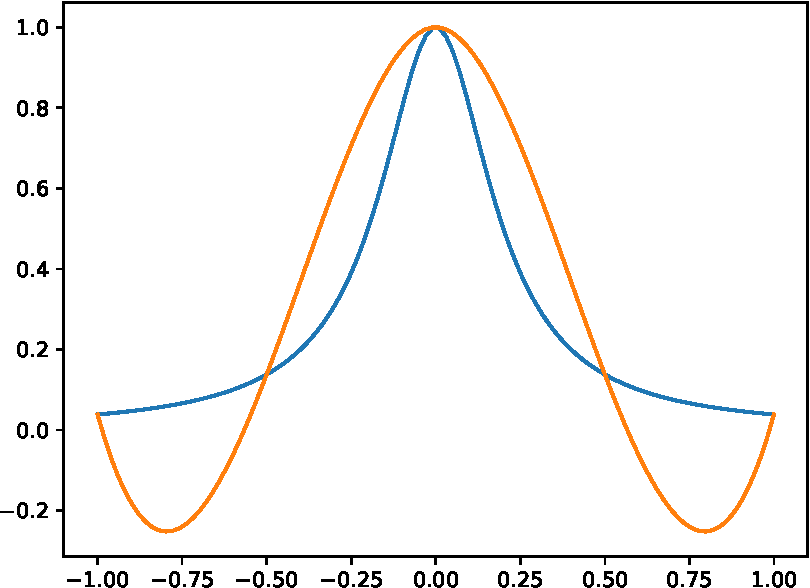
\includegraphics[width = 0.3\textwidth]{chapter_09/exercise_09_51_figure_1.pdf}
  \hspace{1em}
  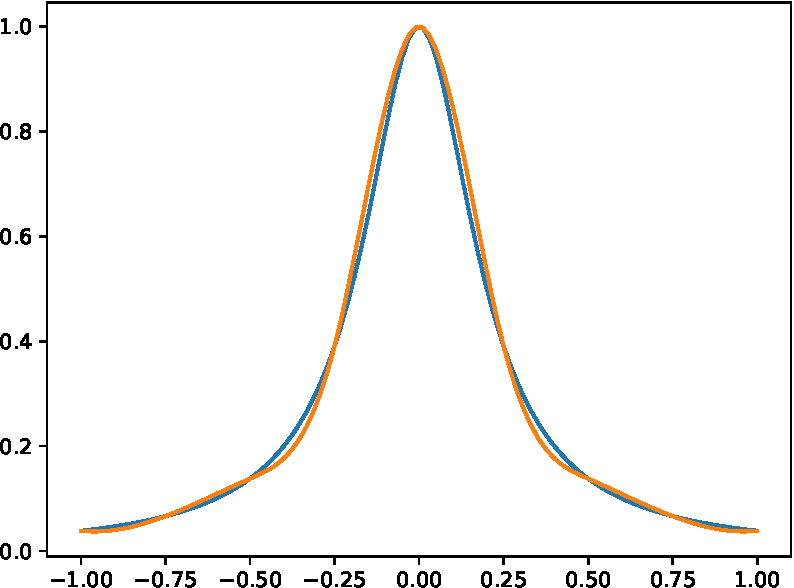
\includegraphics[width = 0.3\textwidth]{chapter_09/exercise_09_51_figure_2.pdf}
  \hspace{1em}
  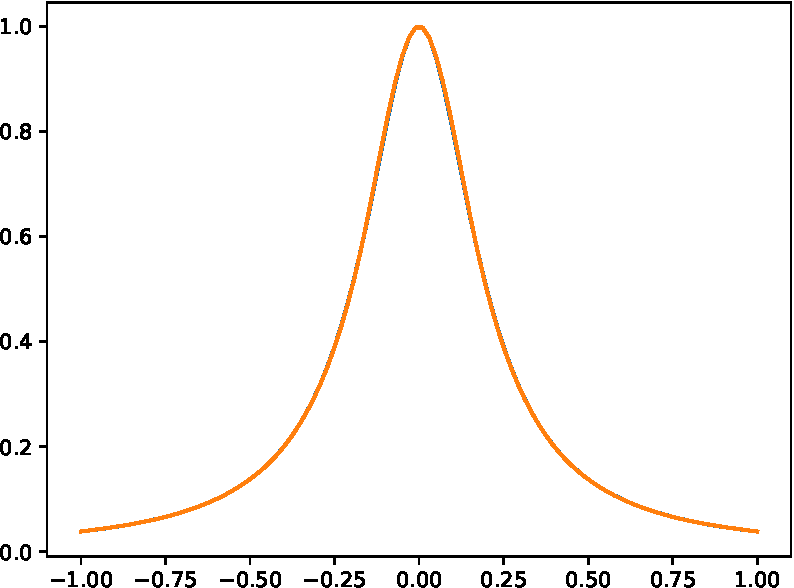
\includegraphics[width = 0.3\textwidth]{chapter_09/exercise_09_51_figure_3.pdf}
\end{center}
